\chapter{Method}
\label{chapter:method}
\epigraph{\textit{Du bist schön, aber dafür kannst du nichts.
Weder Lesen, noch Schreiben, noch was anderes.}}{Alligatoah}
Based on the theory discussed in the previous chapter it is possible to build a model for numerical simulations.
Numerical simulations have been at the heart of fluid dynamics for a long time.
This is mainly because of two statements.
On the one hand we cannot find an analytical solution to every given flow problem, which is due to the shape and the structure of the Navier-Stokes equations.
In fact there are only a few flows that admit an analytical solution. 
They are often referred to as benchmark problems.
One of those is the famous ''Hagen–Poiseuille flow'', see  Sec.~\ref{sec:theory_shallow_water}, which is an analytical solution for a flow field in a canal and was first derived by Poiseuille and Haagen in the 18th century~\cite{suteraHistoryPoiseuilleLaw}.
There are a few other benchmark problems, especially in the low Reynolds number regime with a small or vanishing Stokes number\footnote{The Stokes number is a dimensionless number that defines the behaviour of particles suspended in a flow and can be calculated with $St = \frac{t_0u_0}{l_0}$, where $t_0$ is a relaxation time of the particles, $u_0$ is a characteristic velocity and $l_0$ is a characteristic length scale.}.
The so called Stokes flows admit time reversal symmetry and many have theoretical solutions.
However, not all flows are laminar and in fact most natural flow admit some turbulent behaviour. 
Understanding flows with high Reynolds numbers still poses a problem, or as R. Feynman once said: ''... the most important unsolved problem of classical physics.''

On the other hand solving differential equations with numerical tools is a story of success.
Long before any computer was build, iterative methods for approximating a solution to a given differential or integral equation have been developed.
Leonhard Euler published his findings about what we call today the ''Euler-method'' already in the 18th century~\cite{brezinskiNumericalAnalysisHistorical2012}.
On the blink to the 20$^{\text{th}}$ century Carl Runge and Martin Kutta developed the method nowadays called ''Runge-Kutta Method'' which is of better accuracy than a plain Euler solver~\cite{wBeitragZurNaherungsweisen1901, rungeUeberNumerischeAufloesung1895}.

Several physics problems are being studied to a large extent with numerical tools, e.g., quantum field theory~\cite{montvayQuantumFieldsLattice1994}, solid mechanics~\cite{cardiffThirtyYearsFinite2021}, and as outlined in the introduction Chap.~\ref{chapter:intro}, computational fluid dynamics (CFD) is one of those fields.
Although chip manufacturers have a hard time to keep up with Moore's law, computing power is still growing rapidly~\cite{schallerMooreLawPresent1997}.
Instead of ever faster processors (measured in clock rate), the trend is shifting in the direction of parallel and accelerated computing. 
Throughout the years several accelerator designs emerged.  
One chip design that works particularly well as accelerators are graphics processing units (GPUs).
While a GPU lacks the complexity of a central processing unit (CPU) it excels at doing simple tasks over and over again.
As the name suggests they were initially developed to generate a graphic signal that could be read by a screen. 
It turns out that several algorithms developed for solving differential equations are well suited to be calculated on the GPU. 
Among them is the lattice Boltzmann method, at least a very basic implementation of the method.
GPUs however are not the only devices to be used as accelerators.
Intel for example used a different approach to accelerator computing and already some time ago developed the Xenon Phi.
However with lack of performance as compared to Nvidia's graphics cards and company intern decisions Intel ended the Xenon Phi project in 2020.
The successor of the Xenon Phi project is the very recent \textit{oneAPI} approach and its hardware~\cite{christgauPortingLegacyCUDA2020}.
Shifting the focus towards heterogeneous compute architectures, or as Rick Stevens\footnote{Rick Stevens is Professor at the Department of Computer Science and Associate Laboratory Director, Computing, Environment and Life Sciences at Argonne National Laboratory.} said: ''The future of advanced computing requires heterogeneous hardware to maximize the computing power needed for exascale-class workloads. The oneAPI industry initiative Intel is spearheading will ensure that programming across diverse compute architectures is greatly simplified.''
Not only is this Intel's idea but a general trend in high performance computing (HPC) moving from CPU only clusters to heterogeneous hardware.
Apart from Intel more and more companies joined the development of workload optimized hardware.
Which is possible not only but also due to the technological inventions from ARM (Advanced RISC Machines) and other system on a chip (SoC) design companies.
SoC designs optimized for specific workloads are the key business of ARM, which is a paradigm change of the industry.
For the longest time established chip manufactures also defined the designs of a chips.
Today SoC designs can be manufactured at project manufacturers with TSMC (Taiwan Semiconductor Manufacturing Company Limited) being one of them.
TSMC is also the world leader in the production of semiconductors for computer chips. 
They moved the resolution limit for single transistors from 12nm to about 5nm in roughly 5 years.
These technological steps allowed on the other hand companies such as Apple to design SoCs for their specific needs. 
The M1 Max is from this perspective a very interesting device, although it is not an x86 design. 

Coming up in this chapter is a short overview of numerical methods to iteratively solve the thin film equation, Eq.~(\ref{eq:thin_final}).
Starting with the straightforward finite differences approach and an introduction of the Courant Friedrichs Lewy (CFL) condition~\cite{courantUeberPartiellenDifferenzengleichungen1928}.
We then discuss the possibility to use the bottom up approach and solve Newton's equation of motion for every molecule.
Followed by a short introduction to the main method of this work, the lattice Boltzmann method~\cite{frischLatticeGasAutomataNavierStokes1986, krugerLatticeBoltzmannMethod2017, succiLatticeBoltzmannEquation2001}. 
The mathematical framework as well as its link to kinetic theory will be discussed and the idea of the Chapman-Enskog expansion will be outlined~\cite{chapmanMathematicalTheoryNonuniform1990, enskogKinetischeTheorieVorgange1917}. 
Based on this mathematical model we can define a numerical approach.
Using assumptions, mainly concerning the collision operator, the resulting algorithm is fairly easy to implement and shows good scalability.
This closes the loop with the above statement that the resulting source code is a perfect candidate for GPU programming.

\section{Numerical methods}
\label{sec:numerical_methods}
\begin{figure}
    \centering
    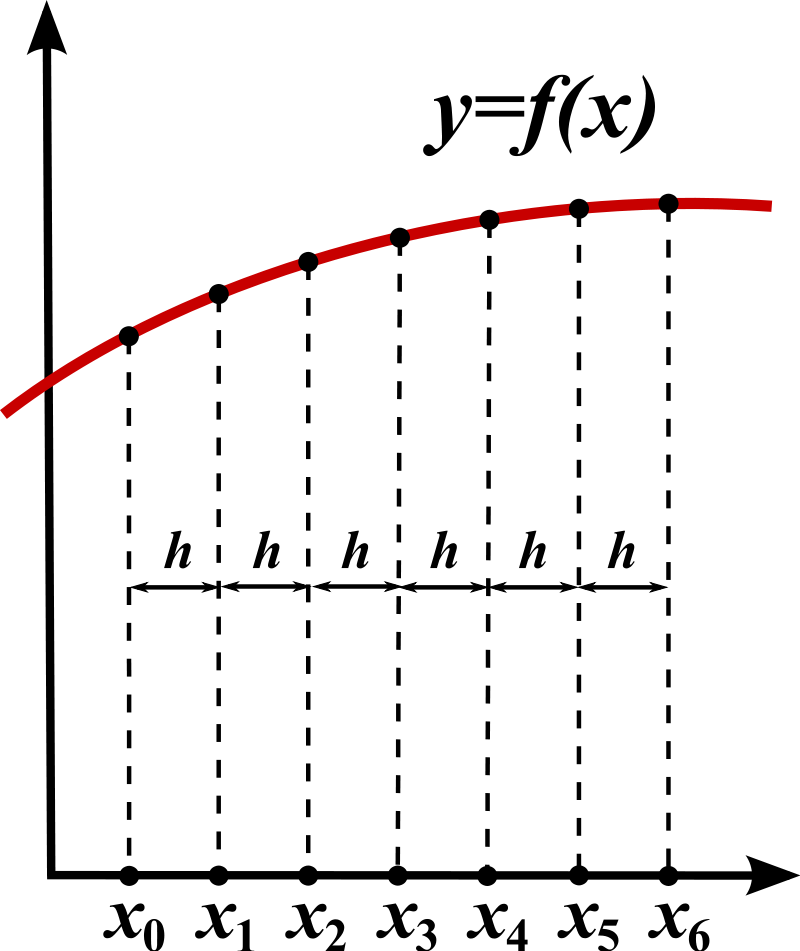
\includegraphics[width=0.5\textwidth]{graphics/800px-Finite_Differences.svg.png}
    \caption{Discretization of a continuous function y (in red) along a discrete space x ($x_0, x_1, x_2$,...).
    Consecutive points on the x-axis are separated by a uniform distance $h$.
    }
    \label{fig:finite_difference}
\end{figure}
The lattice Boltzmann method is one among many to simulate the behaviour of a fluid.
Especially when it comes to numerical simulations of the thin film equation, see Eq.~(\ref{eq:simple_thin_film}), other numerical approaches are more established and have been successfully applied for more than thirty years~\cite{beckerComplexDewettingScenarios2003, peschkaSignaturesSlipDewetting2019, davidovitchSpreadingViscousFluid2005, meckeThermalFluctuationsThin2005, diezGlobalModelsMoving2000, schwartzSimulationDropletMotion1998}.
The thin film equation is a non-linear (stiff) fourth order PDE which requires choosing an appropriate scheme, because not every numerical scheme will be able to provide first stability and second a correct approximation of the solution.
A numerical scheme is a blue print of how to discretize derivatives and arrange terms such that an iterative process converges towards a solution.
That said, developing new numerical schemes for PDEs is still a very active research area.
One way to compute this differential operators on a computer is via finite differences.

\subsection{Finite differences}
Using finite differences means nothing more than discretizing the continuous problem into small (infinitesimal) discrete segments.
Figure~\ref{fig:finite_difference} illustrates a discretization approach where the function $f(x)$ is approximated by a finite set of points which are shown as black dots on the red line.
At every point $x_i$ along the x-axis we know the value of the function $f(x_i)$.
This however does not mean that we know the value of $f(x)$ at arbitrary $x$ values and even worse we do not know $\partial_x f(x_i)$ at $x_i$. 
For a continuous function, e.g., the film thickness $h(\mathbf{x},t)$, we can analytically compute the derivatives. 
Here we are left with a discrete set of points and have yet to come up with an idea to calculate $\nabla h(\mathbf{x}_i, t)$, which is crucial to compute the film pressure, Eq.~(\ref{eq:pfilm}).

Discretization of a derivative is a long studied problem~\cite{booleTreatiseCalculusFinite1872, jordanCalculusFiniteDifferences1965}.
The Taylor expansion gives us a tool to approximate the solution to a differential.
In one spatial dimension there are three different methods to compute the derivative, neglecting boundary conditions there is
\begin{equation}\label{eq:forward_dif}
    \partial_x f(x_i) = \frac{f(x_{i+1}) - f(x_i)}{h},
\end{equation}
where $h$ is the spacing between two consecutive points as introduced in Fig.~\ref{fig:finite_difference}. 
Subtracting the value of the function $f(x_{i+1})$ from $f(x_i)$ is called forward difference.
Changing the interval the backward difference is given as
\begin{equation}\label{eq:backward_dif}
    \partial_x f(x_i) = \frac{f(x_i) - f(x_{i-1})}{h}.
\end{equation}
Both the forward as well as the backward differential are first order in their error, beyond first order is the central difference approach
\begin{equation}\label{eq:center_diff}
    \partial_x f(x_i) = \frac{f(x_{i+1}) - f(x_{i-1})}{2h},
\end{equation}
where the value of the derivative is averaged over a larger interval. 
The second derivative is then simply applying the differential operator (forward, backward, central) to  the first derivative. 
In case of central differences this yields
\begin{equation}\label{eq:second_central_diff}
    \partial_x^2 f(x_i) = \frac{f(x_{i+1})-2f(x_i)+f(x_{i-1})}{^2}.
\end{equation}

However all finite difference schemes suffer from the concrete choice of the discretization, which is often referred to as discretization artifacts.
The starting equation is usually a continuous one in both space and time, but the numerical solver requires a discretized system. 
This can be done as shown in Fig.~\ref{fig:finite_difference} by introducing a grid for the spatial dimensions. 
For now we assume that we can do the same with time and put the temporal dimension into a discrete grid. 
If we take a sine wave and discretize it with an arbitrary grid spacing $h$, that grid spacing will introduce an error to our finite difference scheme. 
We mark two points along the curve and connect them, which yields a straight line. 
Therefore all information in between the points is lost, instead of $y(x) = \sin(x)$ one would guess $y(x) = kx + d$ for the points.
Besides the fact that information about the function is lost it still could be a good enough approximation for the derivative, especially if the points are not too far apart.
Increasing the number of points along the curve, thus making $h$ smaller, will increase the accuracy of the resulting approximation as displayed in Fig.~\ref{fig:finite_difference}.
A good approximation for $y(x) = \sin(x)$ requires therefore more than just two points.
Which explains the so called fidelity of the finite difference method~\cite{guruswamyReviewNumericalFluids2002}.
One needs a fine enough grid to resolve the to be studied dynamics, but the smaller the spacing $h$ gets the more numerically demanding is the calculation.

In fact there are further limitations to the problem of numerically approximating a PDE.
Numerical methods for PDEs, e.g., the thin film or the wave equation, need to satisfy the CFL condition~\cite{courantUeberPartiellenDifferenzengleichungen1928}.  
Beyond other things it states that choosing an increment for time cannot be independent of the spatial resolution.
This condition can be formalized as
\begin{equation}\label{eq:CFL}
    C = \Delta t \left(\sum_{i=1}^n \frac{u_{x_i}}{\Delta x_i}\right) \leq C_{max},
\end{equation}
with $\Delta x_i$ and $\Delta t$ being the spatial and temporal increment, respectively and $u_{x_i}$ being the magnitude of the velocity in the respective direction.
In case of Fig.~\ref{fig:finite_difference} we have $\Delta x = h$. 
Behind this concept is the idea that propagation of information has an upper limit.
For fluid dynamics problems this upper limit is the speed of sound, in electrodynamics it would be the speed of light.
Any propagation larger than this upper limit introduces stability issues.
These issues are purely numerical as we know that air can flow with velocities larger than the speed of sound, however by doing so the flow creates a so called shock.

Thinking of a wave package, numerically it should be ensured that several time iterations are computed before the package has reached the next spatial point of the grid.
The maximal value that the Courant number can reach for an explicit solver, to which for example the lattice Boltzmann method belongs (assuming a BGK collision operator), is $C_{max} = 1$.
For implicit methods the maximal Courant number can be larger than one.
The iteration from $u(x_i,t_0)$ to $u(x_i,t_1)$ is called a time step. 
The ``distance'' between consecutive time values, here $\Delta t = t_1 - t_0$ must ensure that forces and therefore acceleration are well within the stability condition Eq.~(\ref{eq:CFL}).

A very specific finite difference scheme with good stability features is the Crank-Nicolson method~\cite{crankPracticalMethodNumerical1947, pressNumericalRecipes3rd2007}.
This method is second order in time and implicit and has been successfully applied to thin film problems, see for example Refs.~\cite{diezGlobalModelsMoving2000, diezMetallicthinfilmInstabilitySpatially2016, munchDewettingRatesThin2005}.

\subsection{Spectral methods}
Another strategy to solve a differential equation is to perform a transformation.
One rather famous transformation is the Fourier Transformation (FT), which we have used to find the dispersion relation in Sec.~\ref{sec:thin_films} and will encounter again in Chap.~\ref{chapter:second_paper}.
The set of solvers using a FT to solve a given differential equation is called spectral methods.
Doing so has the advantage of interchanging the derivatives with simple multiplications.
For example the term $\partial_x f(x)$ transforms to  
\begin{equation}\label{eq:fourier_transform}
    \partial_x f(x) = q\cdot \tilde{f}(q),
\end{equation}
where $\tilde{f}(q)$ is the Fourier transformed of $f(x)$, e.g., $\tilde{f}(q) = \delta(q - a/2\pi)$ for $f(x) = e^{iax}$. 
Instead of solving a differential equation one solves an algebraic equation, or a set of algebraic equations.
While it is often straightforward to perform the transformation it can become problematic to perform the backward transformation. 
Usually the expressions are fairly complicated and often the backward transformation into real space is not easy to perform.
In Chap.~\ref{chapter:second_paper} we arrive at such an expression for the structure factor $\mathcal{S}(q, t)$.
A structure factor is a measure of the distribution of length scales, roughly speaking.
In this specific case there is no need for a backward transformation because (scattering) experiments usually supply data in Fourier space.

However, when approximating the thin film equation, by iteratively solving an equation, we may be interested in forces, pressures or simply the thickness $h(\mathbf{x},t)$, which is why we need a backward transformation.
Numerically speaking the operators for transformations are matrices, which depend on the specific problem.
Solutions in real space are generated by inversion of these operators and therefore by inversion of an (arbitrary) matrix.
Computing the inverse of a matrix is a demanding problem. 
Nevertheless, these transformation approaches are often quite helpful finding an exact solution.
One rather prominent example is the computation of Green's functions, e.g., in electrostatics~\cite{greenEssayApplicationMathematical1889}.
For the shallow water theory, see Sec.~\ref{sec:theory_shallow_water}, one class of effective methods are the (discontinuous) Galerkin methods~\cite{ernTheoryPracticeFinite2004} and to some extent the related finite element method (FEM).

Literature concerning simulations of the thin film equation using spectral solvers is rather sparse. 
That does however not mean that spectral methods are ill suited for this specific problem.
For example, Dur{\'a}n-Olivencia, M. et al. used a spectral method to approximate the thin film equation. 
Their work also introduced a self-consistent approach to tread thermal fluctuations~\cite{duran-olivenciaInstabilityRuptureFluctuations2019}.

\subsection{Molecular dynamics}
The third approach we discuss in this section is the molecular dynamics method (MD)~\cite{haileMolecularDynamicsSimulation1997, zhangMolecularSimulationThin2019, wengMolecularDynamicsInvestigation2000}.
When we solve the equations of motion of molecules we do not per se think of a \textbf{thin} film flow, however molecular dynamics can be very insightful when dealing with thin film problems. 
In Sec.~\ref{sec:thin_films} we introduced the term wetting and the three phase contact line.
Advancement of the three phase contact line can be boiled down to the interaction between fluid molecules and substrate molecules, therefore MD is perfectly suited to study e.g., slip~\cite{jabbarzadehWallSlipMolecular1999, segaRegularizationSlipLength2013}. 
Instead of working with macroscopic fields, such as density $\rho$ or velocity $\mathbf{u}$, the method uses a bottom up approach.
The main idea is to compute the trajectory of every particle using Newton's equation of motion, therefore to assume that particles are classical objects.
Interactions as well as boundary conditions can be added via pair potentials.
A common interaction potential is the Lennard-Jones potential
\begin{equation}\label{eq:Len-Jon}
    U(r_{ij}) = 4\varepsilon\left[\left(\frac{\sigma}{r_{ij}}\right)^{12}-\left(\frac{\sigma}{r_{ij}}\right)^6\right],
\end{equation}
where $ij$ denotes the particle pair, $\varepsilon$ and $\sigma$ are the model dependent energy and length parameters, respectively.
Clearly this approach is rather elegant.
Knowing the correct values for $\sigma$ and $\varepsilon$, the simulations show good agreement with experiments~\cite{zhangMolecularSimulationThin2019}.

However, there is no free lunch. 
The method is inherently microscopic which makes it compute intensive.
To compute a particle trajectory we need to know where the particle is and how fast it is, thus its position and the velocity.
In a MD simulation we need to know this information for every particle.
While it is possible to arrange this information efficiently, the computation of the pair potential quickly becomes quite resource demanding in terms of computational power.
The results from the computation of pair potentials are forces which act on the particles.
This surmounts to a lot of computational resources for small physical volumes, which is in the context of fluid flows and film formation problematic.
Assuming a box of a few nanometers in all directions and a physical time of about a picosecond ($10^{-12}s$) is already a lot to do for a common laptop.
Clearly a lot is depending on the implementation of the algorithm. 
There are well developed, open source and supported software solutions that not only scale well but have a mature user interface, e.g., LAMMPS and GROMACS~\cite{plimptonFastParallelAlgorithms1995, berendsenGROMACSMessagepassingParallel1995, lindahlGROMACSPackageMolecular2001}.  
However all this development cannot overcome that this method is suited only for relatively small systems and not for macroscopic scales.

Another problem that is inherent to MD simulations is the vast zoo of interaction potentials.
Water for example is not a simple Lennard-Jones liquid, such as liquid Argon. 
Therefore the potential Eq.~(\ref{eq:Len-Jon}) should not be used for water-water interactions.
Although water seems to be a simple molecule with just two hydrogen atoms and one oxygen atom it is in fact a rather complex substance to simulate.
There exists not a single model for how water should interact but several, all with very fine tuned adjustments.
Some include for example the polarity of the water molecule while others neglect it.
Without knowing why a certain water model is more suited than another one, this approach can come down to a black box.
This method therefore requires a lot of literature knowledge and validation with both theory and where possible with experiments.
That said apart from Zhang et al.~\cite{zhangMolecularSimulationThin2019} MD has been used on a diverse set of thin film related problems such as pearling~\cite{koplikPearlingInstabilityNanoscale2006}, dewetting~\cite{bertrandDynamicsDewettingNanoscale2007} or dynamics of droplets~\cite{liuActuatingWaterDroplets2015, wangMolecularDynamicsSimulations2015} to name just a few.

\section{The lattice Boltzmann method}\label{sec:LBM}
\begin{figure}
    \centering
    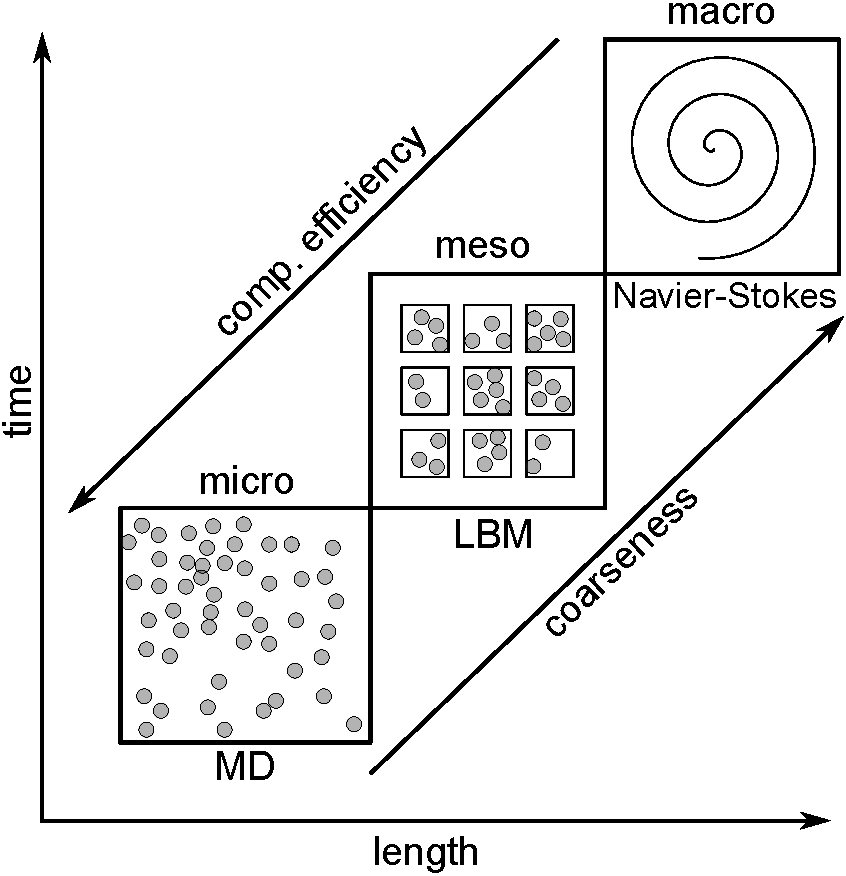
\includegraphics[width=0.55\textwidth]{graphics/Scales_problem.pdf}
    \caption{Schematic display of how different approaches relate to different length and time scales.
    The finer the system is resolved the more computing resources are needed.}
    \label{fig:scales_dummy}
\end{figure}
The lattice Boltzmann method is as the name suggests a discretization approach to the Boltzmann equation~\cite{krugerLatticeBoltzmannMethod2017, succiLatticeBoltzmannEquation2001, wolf-gladrowLatticeGasCellularAutomata2004}.
Boltzmann more then a hundred years ago introduced a model that was build on the assumptions that atoms and molecules move classically.
This was actually just a small portion of his groundbreaking work which forms a whole subsection of physics called statistical mechanics. 
He as well knew that there are a lot of oxygen, nitrogen and other atoms that make up the content of air we inhale with a single breath.
In 1811 already Avogadro calculated that rough number of molecules and around fifty years later Loschmidt came to a similar result~\cite{avagadro1811essai, loschmidtZur1866}:
\begin{equation}
    n = \frac{p N_A}{R T}.
\end{equation}
Here $n$ is the number density, $p$ the pressure, $R$ the gas constant and $T$ the temperature.
The constant named after Avogadro ($N_A$) states that a mole of any substance has about $6 \cdot 10^{23}$ atoms.
Boltzmanns ingenious idea, this adjective is justified as even mathematicians find statistical mechanics appealing, to solve the dynamics of this complex coupled system was to use a statistical ansatz.
Instead of solving the equations of motion for every particle, which is the idea of MD, Boltzmann decided to introduce distribution functions $f(\vec{x},\vec{\xi},t)$, which depend on position, momentum and time and generate an ensemble.
However, to introduce these distribution functions $f(\vec{x},\vec{\xi},t)$ we must make a guess how the atoms or molecules behave in a gas.
We actually shortly discussed one of these guesses in Sec.~\ref{sec:navier_stokes_sec} already. 
The ideal gas is a well working model that assumes that the atoms or molecules in a gas are indistinguishable point particles. 
Furthermore, these particles do not attract or repel each other, neglecting e.g.,~electrostatic forces.
The mean free path of these particles is much larger than their physical size.
Both of these assumptions are actually quite good, because a gas at room temperature and ambient pressure of one bar is a very dilute fluid.
The particles move in random directions with velocities given by a distribution that depends on temperature. 
The only way to transfer energy between particles is via elastic collisions.
This model works exceptionally well for many problems and has been validated experimentally numerous times.
Clearly there are shortcomings to the ideal gas, for example at low temperature and high pressures when intermolecular interactions become important.
However for the scenarios considered in this thesis, the ideal gas serves as a good foundation to the lattice Boltzmann method.

Figure~\ref{fig:scales_dummy} illustrates the idea coming from either a macroscopic system or a microscopic system.
Instead of dealing with every atom or molecule, which is displayed in the bottom left of the figure, it is also possible to use a more coarse approach which is shown in the centre of the figure where distributions over ensembles of particles are used~\cite{raabeOverviewLatticeBoltzmann2004}.
Therefore instead of working in the microscopic world the lattice Boltzmann method works in a mesoscopic regime.
Making it computationally more efficient than e.g., MD for a larger class of problems.
Of course, it is also possible to use a coarser approach and in fact a lot of the classical Navier-Stokes solvers operate in the upper right of Fig.~\ref{fig:scales_dummy}, see Sec.~\ref{sec:Joss_need} for some example solvers.

\subsection{The Boltzmann equation and macroscopic conservation equations}
The dynamics of these distributions $f$ can be formalized and put into an evolution equation which is called the Boltzmann equation
\begin{equation}\label{eq:boltzmann_eq}
    \partial_t f + \vec{\xi}\cdot\vec{\nabla} f + \frac{1}{\rho}\vec{F}\cdot\partial_{\vec{\xi}}f = \Omega(f), 
\end{equation}
where $\vec{\xi}$ is the momentum. 
The first two terms describe the advection of the distribution and the third term measures the effect of a force $\mathbf{F}$ on the momentum~\cite{krugerLatticeBoltzmannMethod2017}.
On the right hand side of the equation is an arbitrarily complex term, the collision operator.
This operator accounts for all collisions the particles perform at any given instance of time.
In principle this operator cannot be computed analytically, because one would need to take into account all possible collision terms from two up to n-point interactions.

However with a smart ansatz it is possible to find a suitable approximation to the collision operator.
One ansatz we can make is,
\begin{enumerate}
    \item The state of the fluid is not far from its equilibrium.
    \item During the collision it approaches its equilibrium with a relaxation time $\tau$.
\end{enumerate}
Bhatnagar, Gross and Krook (BGK) were the first ones who worked out the mathematical model behind this ansatz~\cite{bhatnagarModelCollisionProcesses1954}.
This model can be formalized quite simply and reads
\begin{equation}\label{eq:operator_bgk}
    \Omega(f) = -\frac{1}{\tau}(f - f^{eq}),
\end{equation}
where $f^{eq}$ denotes the equilibrium distribution function,
\begin{equation}\label{eq:boltzmann_eq_dist}
    f^{eq}(\vec{x}, |\vec{v}|, t) = \rho\left(\frac{1}{2\pi R T}\right)^{3/2} e^{-|\vec{v}|^2/(2RT)},
\end{equation}
which is called Maxwell-Boltzmann distribution.
The moments of the BGK collision operator satisfy the following set of equations
\begin{align}
    \int \Omega(f) \diff^3\xi = 0, \label{eq:BGK_1}\\
    \int \vec{\xi}\Omega(f) \diff^3\xi = \vec{0}, \label{eq:BGK_2}\\
    \int |\vec{\xi}|^2\Omega(f) \diff^3\xi = 0, \label{eq:BGK_3}\\
    \int |\vec{v}|^2\Omega(f) \diff^3\xi = 0. \label{eq:BGK_4}
\end{align}
The first of the above equations states that the mass is conserved, while Eq.~(\ref{eq:BGK_2}) ensures momentum conservation.
Eqs.~(\ref{eq:BGK_3}, \ref{eq:BGK_4}) tell us that both that the total energy as well as the internal energy are conserved.
Note that $\vec{v}$ is a relative velocity which measures the deviation $\vec{v}(\vec{x}, t) = \vec{\xi}(\vec{x}, t) - \vec{u}(\vec{x}, t)$.

Taking these four constraints into consideration as well as the two points above one finds that the BGK operator is the simplest one to satisfy them all.
With one side note however: The full collision operator from Boltzmann does predict a different Prandtl number ($Pr$) than the BGK approximation.
The Prandtl number $Pr = \nu/\alpha$ measures viscosity against thermal diffusivity ($\alpha$). 
Using BGK one gets $Pr=1$ while monoatomic gases or Boltzmann's operator showing $Pr\simeq 2/3$~\cite{cercignaniBoltzmannEquation1988, krugerLatticeBoltzmannMethod2017}.

The Boltzmann equation, Eq.~(\ref{eq:boltzmann_eq}), was developed as an evolution for a gas and is build upon distributions of microscopic particles, e.g., Eq.~(\ref{eq:boltzmann_eq_dist}).
Using the BGK approximation for the collision operator we found that its moments conserve mass, momentum and energy.
The next step is to show that the Boltzmann equation with the BGK operator obeys macroscopic conservation equations, as such Eq~(\ref{eq:cont_3}) and Eq.~(\ref{eq:navier_stokes_fin}).
For the mass conservation we compute the zeroth moment of Eq.~(\ref{eq:boltzmann_eq}), therefore integrating it over the velocity space
\begin{equation}\label{eq:boltzmann_mass_cons}
    \partial_t\int f\diff^3\xi + \partial_{x_{\beta}}\int\xi_{\beta} f\diff^3\xi + \frac{F_{\beta}}{\rho}\int\partial_{\xi_{\beta}}f\diff^3\xi = \int\Omega(f)\diff^3\xi,
\end{equation}
with moments of $f$ given by
\begin{align}
    \Pi_0 = \int f\diff^3\xi = \rho, \label{eq:boltzmann_moment_1}\\
    \Pi_{\alpha} = \int\xi_{\alpha} f\diff^3\xi = \rho u_{\alpha}, \label{eq:boltzmann_moment_2}\\
    \Pi_{\alpha\beta} = \int\xi_{\alpha}\xi_{\beta} f\diff^3\xi, \label{eq:boltzmann_moment_3}\\
    \Pi_{\alpha\beta\gamma} = \int\xi_{\alpha}\xi_{\beta}\xi_{\gamma} f\diff^3\xi. \label{eq:boltzmann_moment_4}
\end{align}
From Eq.~\ref{eq:BGK_1} we know that the right hand side of Eq.~(\ref{eq:boltzmann_mass_cons}) is zero, furthermore the force term is vanishing as well, because~\cite{krugerLatticeBoltzmannMethod2017} 
\begin{equation}
    \int\partial_{\xi_{\beta}}f\diff^3\xi = 0.
\end{equation}
The non vanishing contributions, thus the first two integrals on the left hand side are given by Eqs.~(\ref{eq:boltzmann_moment_1}-\ref{eq:boltzmann_moment_2}) and therefore we get
\begin{equation}\label{eq:mass_boltzmann}
    \partial_t \rho + \partial_{x_{\beta}}(\rho u_{\beta}) = 0, 
\end{equation}
which is the macroscopic continuity equation, see Eq.~(\ref{eq:cont_3}).
This is actually a quite remarkable result, because we did not need to specify $f$ during this derivation and therefore any distribution function $f$ satisfies mass conservation.

For the momentum conservation we take the first moment of Eq.~(\ref{eq:boltzmann_eq}), thus we multiply with $\xi$ and integrate
\begin{equation}
    \partial_t\int\xi_{\alpha}f\diff^3\xi + \partial_{x_{\beta}}\int\xi_{\alpha}\xi_{\beta} f\diff^3\xi + \frac{F_{\beta}}{\rho}\int\xi_{\alpha}\partial_{\xi_{\beta}}f\diff^3\xi = \int\xi_{\alpha}\Omega(f)\diff^3\xi.
\end{equation}
The right hand side is vanishing according to Eq.~(\ref{eq:BGK_2}). 
The first two integrals on the left hand side can be found from Eqs.~(\ref{eq:boltzmann_moment_2}-\ref{eq:boltzmann_moment_3}).
For the force term we use integration by parts and get
\begin{equation}
    \int\xi_{\alpha}\partial_{\xi_{\beta}}f\diff^3\xi = -\int\partial_{\xi_{\beta}}\xi_{\alpha} f\diff\xi^3 = -\rho\delta_{\alpha\beta}.
\end{equation}
Collecting the non zero contribtuions we have
\begin{equation}\label{eq:boltzmann_mom_cons}
    \partial_t (\rho u_{\alpha}) + \partial_{x_{\beta}}(\Pi_{\alpha\beta}) = F_{\alpha}, 
\end{equation}
with $\Pi_{\alpha\beta}$ being the momentum flux tensor, which can be decomposed into
\begin{equation}\label{eq:mom_flux_tensor_1}
    \Pi_{\alpha\beta} = \rho u_{\alpha}u_{\beta} +\int v_{\alpha}v_{\beta}f\diff^3\xi,
\end{equation}
with 
\begin{equation}\label{eq:mom_flux_tensor_2}
    \sigma_{\alpha\beta} = -\int v_{\alpha}v_{\beta}f\diff^3\xi,
\end{equation}
being a stress tensor.
Inserting Eqs.(\ref{eq:mom_flux_tensor_1}-\ref{eq:mom_flux_tensor_2}) into Eq.~(\ref{eq:boltzmann_mom_cons}) we have,
\begin{equation}\label{eq:mom_boltzmann}
    \partial_t (\rho u_{\alpha}) + \partial_{x_{\beta}}(\rho u_{\alpha}u_{\beta}) = \partial_{x_{\beta}}\sigma_{\alpha\beta} + F_{\alpha}.
\end{equation}
This equation is rather similar to Eq.~(\ref{eq:navier_stokes_2}) or Eq.~(\ref{eq:navier_stokes_fin}), however we cannot solve it yet as we are not able to compute the stress tensor without further knowledge about $f$.

For completeness let us also compute the energy conservation. 
We therefore multiply Eq.~(\ref{eq:boltzmann_eq}) with $\xi_{\alpha}\xi_{\alpha}$, thus the trace of the second moment, and integrate
\begin{equation}\label{eq:boltzmann_energy_cons}
    \partial_t\int\xi_{\alpha}\xi_{\alpha}f\diff^3\xi + \partial_{x_{\beta}}\int\xi_{\alpha}\xi_{\alpha}\xi_{\beta} f\diff^3\xi + \frac{F_{\beta}}{\rho}\int\xi_{\alpha}\xi_{\alpha}\partial_{\xi_{\beta}}f\diff^3\xi = \int\xi_{\alpha}\xi_{\alpha}\Omega(f)\diff^3\xi.
\end{equation}
The collision term vanishes again and for the force term we apply integration by parts once more,
\begin{equation}
    \int\xi_{\alpha}\xi_{\alpha}\partial_{\xi_{\beta}}f\diff^3\xi = -\int\partial_{\xi_{\beta}}(\xi_{\alpha}\xi_{\alpha})f\diff^3\xi = -2\rho u_{\beta}.
\end{equation}
Collecting all non zero terms yields
\begin{equation}
    \partial_t(\rho E) + \frac{1}{2}\partial_{x_{\beta}}\Pi_{\alpha\alpha\beta} = F_{\beta}u_{\beta},
\end{equation}
where $\rho E$ is the total energy density.
Decomposing $\Pi_{\alpha\alpha\beta}$ similarly to Eq.~(\ref{eq:mom_flux_tensor_1}) we find
\begin{equation}
    \partial_t(\rho E) + \partial_{x_{\beta}}(\rho u_{\beta}E) = \partial_{x_{\beta}}(u_{\alpha}\sigma_{\alpha\beta}) + F_{\beta}u_{\beta} -\partial_{x_{\beta}}q_{\beta},
\end{equation}
where we used
\begin{equation}\label{eq:boltzmann_heat_flux}
    q_{\beta} = \int v_{\alpha}v_{\alpha}v_{\beta}f\diff^3\xi, 
\end{equation}
with $\vec{q}$ being the heat flux.

Both the stress tensor, Eq.~(\ref{eq:mom_flux_tensor_2}), and the heat flux, Eq.~(\ref{eq:boltzmann_heat_flux}), cannot be derived without specifying $f$.
However, the only distribution we have readily available is the equilibrium distribution $f^{eq}$, Eq.~(\ref{eq:boltzmann_eq_dist}).
This marks the starting point for the famous Chapman-Enskog expansion, which was derived around a hundred years ago~\cite{chapmanMathematicalTheoryNonuniform1990, enskogKinetischeTheorieVorgange1917}. 
The idea is to use a perturbative expansion for $f$ around $f^{eq}$ and $\partial_t$, 
\begin{equation}\label{eq:chap-ens-expansion}
    f = f^{eq} + \epsilon f^{(1)} + \epsilon^2 f^{(2)} + O(\epsilon^3),\quad \partial_t = \partial_{t_0} + \epsilon\partial_{t_1} + O(\epsilon^2),
\end{equation}
where $\epsilon\approx Kn$ and $Kn$ is the Knudsen number\footnote{$Kn = \lambda/L$ is a measure to compare the mean free path to a characteristic length scale, i.e. ballistic and diffusive regime.}. 
Already at zeroth order, therefore $f \approx f^{eq}$, we find that Eq.~(\ref{eq:mom_boltzmann}) resembles the Euler equation, Eq.~(\ref{eq:navier_stokes_2}), from Sec.~\ref{sec:navier_stokes_sec}.
The time scale $t_0$ can be undestood as advective time scale while $t_1$ marks the diffusive time scale~\cite{dellarNonhydrodynamicModesPriori2002}.
The missing viscous contributions are not covered by the zeroth order.
However already at first order of the expansion, thus $f\approx f^{eq} + \epsilon f^{(1)}$, the Navier-Stokes equation can be recovered~\cite{chenLatticeBoltzmannMethod1998}.
In the next section we use this result and discretize the Boltzmann equation with the BGK operator.

\subsection{From continuum to discrete lattice fields} 
\begin{figure}
    \centering
    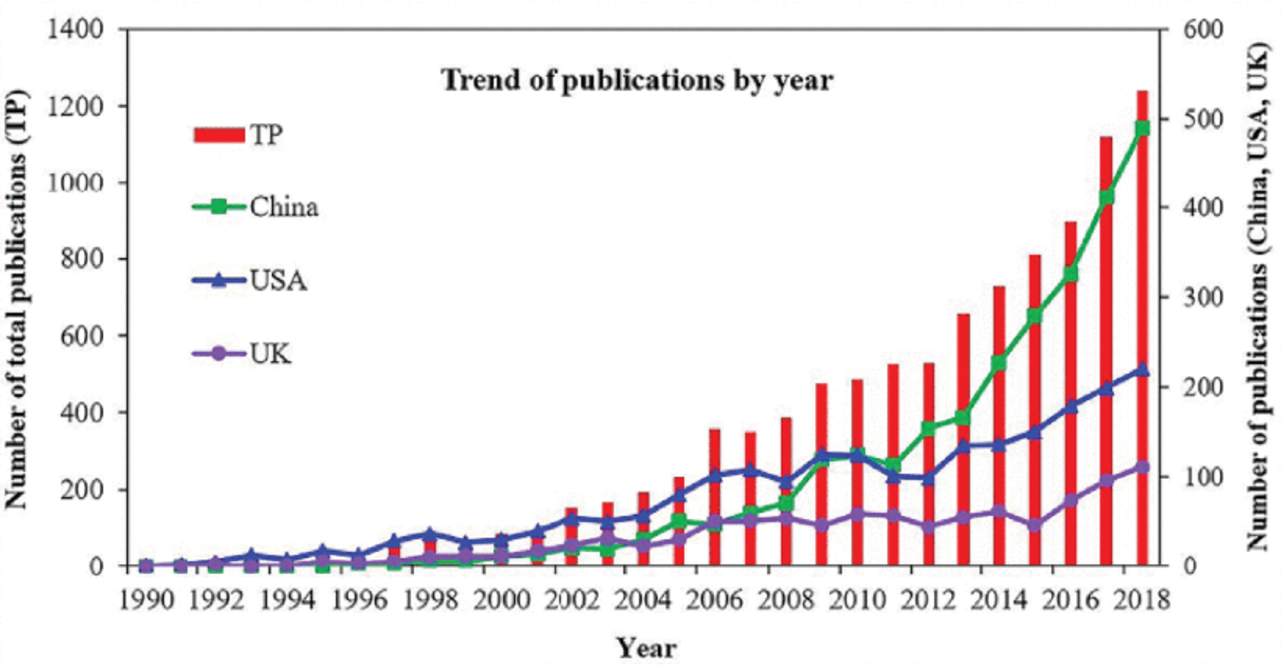
\includegraphics[width=0.75\textwidth]{graphics/lbm_citations.pdf}
    \caption{Number of lattice Boltzmann method related publications measured from 1990 to 2018 according to Ref.~\cite{liLatticeBoltzmannMethod2020}.
    The red bars indicate the total number of publications per year. 
    The green, blue and lavender lines show the number of publications for the most ``productive'' countries, respectively China, USA and the UK.}
    \label{fig:lbm_cite}
\end{figure}

In 1986 Frisch, Hasslacher and Pomeau published their groundbreaking article on the simulation of the Navier-Stokes equation using lattice gas automata (LGA)~\cite{frischLatticeGasAutomataNavierStokes1986}.
The LGA model is in contrast to the lattice Boltzmann method a purely boolean model, thus a lattice site hosts a particle or not~\cite{mcnamaraUseBoltzmannEquation1988}.
Due to the usage of boolean states the simulations suffered a serious noise problem.

The lattice Boltzmann method is the successor of the LGA, where among other things the boolean lattice state was abandoned in favour of a distribution function $f_{i}(\vec{x}, t)$ which in simulations is represented by a real number~\cite{chenLatticeBoltzmannMethod1998}. 
Since the method got first developed in the late 1980s it has gained more and more popularity, as shown in Fig.~\ref{fig:lbm_cite}~\cite{liLatticeBoltzmannMethod2020}.
Due the simplicity of the method a lot has been worked out over last forty years.
The reason why the lattice Boltzmann method is lacking behind when it comes to thin film flows is due to its origin as an approximation to the Navier-Stokes equation.
That said, there are of course numerous studies of wetting and sliding droplets using the lattice Boltzmann method, e.g., Sbragaglia et al.~\cite{sbragagliaSlidingDropsAlternating2014}.
However they rely on additional contributions for either multiphase or multicomponent models~\cite{shanLatticeBoltzmannModel1993, chenLatticeMethodsTheir1995, shanKineticTheoryRepresentation2006}.

The discretization of Eq.~(\ref{eq:boltzmann_eq}) using the lattice Boltzmann method is straightforward and does not require complex meshing.
In fact this is one of the strengths the lattice Boltzmann method inherited from the LGA.
As the name suggests a lattice with lattice constants $\Delta x$ and $\Delta t$ for spatial and temporal discretization is the desired numerical domain. 
The discretized Boltzmann equation without force term reads,
\begin{equation}\label{eq:LBM_discret_noforces}
    f_i(\vec{x}+\vec{c}_i\Delta t, t+ \Delta t) - f_i(\vec{x}, t) = -\frac{\Delta t}{\tau}(f_i(\vec{x}, t) - f^{eq}_i(\vec{x}, t)),
\end{equation}
where the $\vec{c}_{i}$ form a discrete set of $\alpha$ velocities that upon symmetry considerations replace $\vec{\xi}$ of the previous section~\cite{rubinsteinTheoryLatticeBoltzmann2008}.
This equation is also called lattice Boltzmann equation (LBE). 
The perturbative expansion around the equilibrium distribution, Eq.~(\ref{eq:chap-ens-expansion}) does also hold for a discretized velocity space, therefore
\begin{equation}\label{eq:expansion_f}
    f_i = f_i^{eq} + \epsilon f_i^{(1)} + \epsilon^2 f_i^{(2)} + O(\epsilon^3).
\end{equation}
Introducing the non-equilibrium part of the discretized distribution $f_{i}$ as $f_i^{neq} = f_i - f_i^{eq}$. 
From Eqs.~(\ref{eq:BGK_1}-\ref{eq:BGK_2}) we know that the non-equilibrium part has to satisfy, 
\begin{align}\label{eq:non_constraint}
    \sum_i f_i^{neq} = 0, \\
    \sum_i \vec{c}_i f_i^{neq} = \vec{0}, 
\end{align}
where due to discretization the integral becomes a sum.
The moments of the equilibrium functions obey the following relations~\cite{chenLatticeBoltzmannMethod1998} 
\begin{align}
    \Pi^{eq} &= \sum_{i} f_{i}^{eq} = \rho, \label{eq:moments_equilibria_1}\\
    \Pi^{eq}_{\alpha} &= \sum_i c_{i\alpha}f_i^{eq} = \rho u_{\alpha}, \label{eq:moments_equilibria_2}\\
    \Pi^{eq}_{\alpha\beta} &= \sum_{i} c_{i\alpha} c_{i\beta}f_i^{eq} = \rho u_{\alpha} u_{\beta} + \rho c_s^2\delta_{\alpha\beta}, \label{eq:moments_equilibria_3}\\
    \Pi^{eq}_{\alpha\beta\gamma} &= \sum_i c_{i\alpha} c_{i\beta} c_{i\gamma}f_i^{eq} = \rho c_s^2(u_{\alpha}\delta_{\beta\gamma} + u_{\beta}\delta_{\gamma\alpha} + u_{\gamma}\delta_{\alpha\beta}), \label{eq:moments_equilibria_4}
\end{align}
where the Greek indices refer to the spatial dimensions $(x,y,z)$. 
For the zeroth and first moment we also require that
\begin{align}
    \sum_{i} f_{i}^{eq} &= \sum_{i} f_{i} = \rho, \\
    \sum_i c_{i\alpha}f_i^{eq} &= \sum_i c_{i\alpha}f_i = \rho u_{\alpha}.
\end{align}
Clearly Eqs.~(\ref{eq:moments_equilibria_1}-\ref{eq:moments_equilibria_4}) resemble Eqs.~(\ref{eq:boltzmann_moment_1}-\ref{eq:boltzmann_moment_4}) at zeroth order of Eq.~(\ref{eq:expansion_f}).
As a solvability condition for the upcoming derivation we use,
\begin{align}
    \sum_{i} f_{i}^{(n)} = 0, \label{eq:all_order_constraint_1}\\
    \sum_{i} \vec{c}_{i}f_{i}^{(n)} = \vec{0},  \label{eq:all_order_constraint_2}
\end{align}
which basically ensures mass and momentum conservation of the collision operator.

Performing a Taylor expansion of Eq.~(\ref{eq:boltzmann_eq}) with a discrete set of velocities assuming no force is present yields~\cite{krugerLatticeBoltzmannMethod2017}
\begin{equation}\label{eq:Taylor_discret_boltzmann}
    \Delta t (\partial_t + c_{i\alpha}\partial_{\alpha})f_{i} + \frac{\Delta t^2}{2}(\partial_t + c_{i\alpha}\partial_{\alpha})^2 f_{i} + O(\Delta t^3) = -\frac{\Delta t}{\tau} f_{i}^{neq}.
\end{equation}
Leaving higher orders aside one finds that this is actually a slow mode expansion of $f_{i}$.
The distribution functions $f_{i}$, therefore only change on macroscopic time scales. 
If this statement is violated higher orders need to be considered.
Subtracting $\Delta t/2 (\partial_t + c_{i\alpha}\partial_{\alpha})$ from both sides yields
\begin{equation}\label{eq:derive_lbm_orders}
    \Delta t (\partial_t + c_{i\alpha}\partial_{\alpha})f_{i} = -\frac{\Delta t}{\tau} f_{i}^{neq} + \Delta t (\partial_t + c_{i\alpha}\partial_{\alpha})\frac{\Delta t}{2\tau} f^{neq}_{i},
\end{equation}
which is first order in derivatives.
Here we use the second expansion of Eq.~(\ref{eq:chap-ens-expansion}) and expand the time derivative in orders of $Kn$,
\begin{equation}\label{eq:expansion_time}
    \Delta t \partial_t f_{i} = \Delta t (\epsilon\partial_t^{(1)} + \epsilon^2\partial_t^{(2)} + O(\epsilon^3)) f_{i}.
\end{equation}
For the spatial deviates it is sufficient to use
\begin{equation}\label{eq:expansion_space}
    \Delta t c_{i\alpha}\partial_{\alpha} f_{i} = \Delta t(\epsilon c_{i\alpha}\partial_{\alpha}^{(1)}) f_{i}.
\end{equation}
With a note of caution for Eq.~(\ref{eq:expansion_time}) as only the sum of all orders in $\epsilon$ resembles the real time derivative.
Applying both expansions Eq.~(\ref{eq:expansion_f}) and Eq.~(\ref{eq:expansion_time}) to Eq.~(\ref{eq:derive_lbm_orders}) we have
\begin{equation}\label{eq:first_order_esp}
    (\partial_t^{(1)} + c_{i\alpha}\partial_{\alpha}) f_{i}^{eq} = -\frac{\Delta t}{\tau} f_{i}^{(1)}
\end{equation}
at first order in $\epsilon$ and 
\begin{equation}\label{eq:sec_order_esp}
    \partial_t^{(2)} f_{i}^{eq} + (\partial_t^{(1)} + c_{i\alpha}\partial_{\alpha})\left(1 - \frac{\Delta t}{2\tau}\right) f_{i}^{(1)} = -\frac{\Delta t}{\tau} f_{i}^{(2)},
\end{equation}
for $O(\epsilon^2)$.

Taking the moments of Eq.~(\ref{eq:first_order_esp}), see Eqs.(\ref{eq:moments_equilibria_1}-\ref{eq:moments_equilibria_4}) yields
\begin{align}
    \partial_t^{(1)}\rho + \partial_{\beta}^{(1)}(\rho u_{\beta}) &= 0, \label{eq:cont_lbm}\\
    \partial_t^{(1)}(\rho u_{\alpha}) + \partial_{\beta}^{(1)}\Pi^{eq}_{\alpha\beta} &= 0, \label{eq:mom_lbm}\\
    \partial_t^{(1)}\Pi^{eq}_{\alpha\beta} + \partial_{\gamma}^{(1)}\Pi^{eq}_{\alpha\beta\gamma} &= -\frac{1}{\tau}\Pi^{(1)}_{\alpha\beta}, \label{eq:energy_lbm}
\end{align}
for which the moments $\Pi$ are
\begin{align}
    \Pi^{eq}_{\alpha\beta} &= \sum_{i}c_{i\alpha} c_{i\beta} f_{i}^{eq} = \rho u_{\alpha} u_{\beta} + \rho c_s^2\delta_{\alpha\beta}, \label{eq:Pi_lbm_1}\\
    \Pi^{eq}_{\alpha\beta\gamma} &= \sum_{i}c_{i\alpha} c_{i\beta} c_{i\gamma} f_{i}^{eq} = \rho c_s^2(u_{\alpha}\delta_{\beta\gamma} + u_{\beta}\delta_{\gamma\alpha} + u_{\gamma}\delta_{\alpha\beta}), \label{eq:Pi_lbm_2}\\
    \Pi^{(1)}_{\alpha\beta} &= \sum_{i}c_{i\alpha} c_{i\beta} f_{i}^{(1)}, \label{eq:Pi_lbm_3}
\end{align}
where Eqs.~(\ref{eq:moments_equilibria_1}-\ref{eq:moments_equilibria_4}) have been used.
Similar to Eq.~(\ref{eq:mass_boltzmann}) and Eq.~(\ref{eq:mom_boltzmann}) the discretized equations, therefore Eq.~(\ref{eq:cont_lbm}) and Eq.~(\ref{eq:mom_lbm}) resemble the continuity and Euler momentum equation.

Computing the moments of Eq.~(\ref{eq:sec_order_esp}) we have
\begin{align}
    \partial_t^{(2)}\rho &= 0, \\
    \partial_t^{(2)}(\rho u_{\alpha}) + \partial^{(1)}_{\beta}\left(1 - \frac{\Delta t}{2\tau}\right)\Pi_{\alpha\beta}^{(1)} &= 0.
\end{align}
As there is now an equation for $\Pi^{(1)}_{\alpha\beta}$ it is possible to collect the mass and momentum equation for both $O(\epsilon)$ and $O(\epsilon^2)$
\begin{align}
    (\epsilon\partial_t^{(1)} + \epsilon^2\partial^{(2)})\rho + \epsilon\partial_{\alpha}^{(1)}(\rho u_{\alpha}) &= 0, \label{eq:Navier_stokes_01}\\
    (\epsilon\partial_t^{(1)} + \epsilon^2\partial^{(2)})(\rho u_{\alpha}) + \epsilon\partial_{\beta}^{(1)}\Pi^{eq}_{\alpha\beta} &= -\epsilon^2\partial_{\beta}^{(1)}\left(1 - \frac{\Delta t}{2\tau}\right) \Pi^{(1)}_{\alpha\beta}. \label{eq:Navier_stokes_02}
\end{align}
This system in fact resembles the Navier-Stokes equation with the small pitfall that the viscous stress tensor
\begin{equation}
    \sigma = - \left(1 - \frac{\Delta t}{2\tau}\right) \Pi^{(1)},
\end{equation}
is as of now still unknown.
Cut the last part short for an isothermal equation of state and $f_{i}^{eq}$ as function of $O(u^2)$ for example
\begin{equation}\label{eq:eqi_dist1}
    f_{i}^{eq} = \rho(a + b c_{i\alpha} u_{\alpha} + d (c_{i\alpha} u_{\alpha})^2 + e u^2),
\end{equation}
where $a, b, d, e$ are unkown constants~\footnote{In this alphabetic order $c$ is left out to avoid confusion with the lattice velocities.} then the tensor is given as
\begin{equation}\label{eq:stress_first_order}
    \Pi^{(1)} = -\rho c_s^2\tau(\partial_{\beta}^{(1)}u_{\alpha} + \partial_{\alpha}^{(1)}u_{\beta}) + \tau\partial_{\gamma}^{(1)}(\rho u_{\alpha} u_{\beta} u_{\gamma}),
\end{equation}
which concludes the expansion part.
The continuity and the Navier-Stokes equation can be derived by inserting Eq.~{\ref{eq:stress_first_order}} into Eqs.~(\ref{eq:Navier_stokes_01}-\ref{eq:Navier_stokes_02}) and reverting the expansion such that,
\begin{align}
    \partial_t\rho + \partial_{\gamma}(\rho u_{\gamma}) &= 0, \\
    \partial_t(\rho u_{\alpha} + \partial_{\beta}(\rho u_{\alpha}u_{\beta}) &= -\partial_{\alpha}p + \partial_{\beta}[\eta(\partial_{\beta}u_{\alpha} +\partial_{\alpha}u_{\beta})],
\end{align}
where we have neglected the $O(u^3)$ (error) term and used $p = \rho c_s^{2}$ as well as $\eta = \rho c_s^{2}\left(\tau - \frac{\Delta t}{2}\right)$~\cite{krugerLatticeBoltzmannMethod2017}.

So far however no assumptions on the lattice distributions are made and the discrete equilibrium distribution function has not been specified.
Paving work by He and Luo as well as group theoretical arguments derived by Rubinstein and Luo showed that based on dimensionality just a few (discrete) velocities are sufficient~\cite{heTheoryLatticeBoltzmann1997, rubinsteinTheoryLatticeBoltzmann2008}.
In fact in Chap.~\ref{chapter:first_paper} all numerical experiments were performed on a D2Q9 lattice therefore $\mathbf{c}_{i}$ is
\begin{equation}\label{eq:speeds_method}
\mathbf{c}_{i}  =
\left\{
\begin{array}{ll}
(0,0) & \alpha = 0, \\
\left[\cos{\frac{(i-1)\pi}{4}}, \sin{\frac{(i-1)\pi}{4}} \right] &  i=1,3,5,7 \\
\sqrt{2}\left[\cos{\frac{(i-1)\pi}{4}}, \sin{\frac{(i-1)\pi}{4}} \right] & i=2,4,6,8~,
\end{array}
\right.    
\end{equation}
The only missing pieces are $a, b, c, d$ of Eq.~(\ref{eq:eqi_dist1}).
Using the set of equations~(\ref{eq:moments_equilibria_1}-\ref{eq:moments_equilibria_4}) one quickly finds
\begin{equation}
    a = 1,\quad b = \frac{1}{c_s^2},\quad d = \frac{1}{2c_s^4},\quad e = \frac{1}{2c_s^2},
\end{equation}
with lattice weights
\begin{equation}\label{eq:weightsD2Q9_meth}
w_{i} = \begin{cases}
4/9 &\text{$i = 0$}\\
1/9 &\text{$i = 1,2,3,4$}\\
1/36 &\text{$i = 5,6,7,8$}
\end{cases}
,
\end{equation}
such that the equilibria can be written as
\begin{equation}\label{eq:eqi_dist2}
    f_{i}^{eq} = w_{i}\rho\left(1 + \frac{c_{i\alpha} u_{\alpha}}{c_s^2} +  \frac{(c_{i\alpha} u_{\alpha})^2}{2c_s^4} + \frac{u^2}{2c_s}\right).
\end{equation}
Together with the evolution equation Eq.~(\ref{eq:LBM_discret_noforces}) it is therefore possible to approximate the Navier-Stokes equation, at least in regimes of small Knudsen and Mach numbers, $Kn \ll 1$ and $Ma \ll 1$.

Many articles about the lattice Boltzmann method mention a collision step and a streaming step.
This can be achieved by splitting Eq.~(\ref{eq:LBM_discret_noforces}) into a purely local part, 
\begin{equation}\label{eq:collision_step}
    f^{\star}_i(\vec{x},t) = \left(1-\frac{\Delta t}{\tau}\right)f_i(\vec{x},t) + \frac{\Delta t}{\tau}f_i^{eq}(\vec{x},t),
\end{equation}
and a non-local propagation step
\begin{equation}\label{eq:steaming_step}
    f_i(\vec{x}+\vec{c}_i\Delta t,t + \Delta t) = f^{\star}_i(\vec{x},t).
\end{equation}
This rearrangement offers a unique computational advantage, because Eq.~(\ref{eq:collision_step}) is perfectly suited for parallel computation.

\subsection{The shallow water equations on the lattice}\label{susbsec:shallow_water_lattice_boltzmann}

The idea however of this thesis is not to approximate the Navier-Stokes equation but to have a numerical solver for the thin film equation.
As outlined in Sec.~\ref{sec:theory_shallow_water} there is a system which has some similarities with the thin film equation, namely the shallow water equations, Eqs.~(\ref{eq:shallow_water_01}-\ref{eq:shallow_water_02}). 
In fact it is possible to derive with a similar ansatz, the shallow water equations from the Boltzmann equation~\cite{salmonLatticeBoltzmannMethod1999, zhouLatticeBoltzmannMethods2004, dellarNonhydrodynamicModesPriori2002}.
The starting point are the two equations for mass and momentum conservation from Sec.~\ref{sec:theory_shallow_water},
\begin{align}
    \partial_t h + \partial_{x_{\alpha}}(u_{\alpha}h) = 0, \label{eq:lbe_shallow_cont}\\
    \partial_t (u_{\alpha}h) + \partial_{x_{\beta}}(P_{\alpha\beta} - \mathcal{S}_{\alpha\beta}) = 0, \label{eq:lbe_shallow_mom}
\end{align}
where $\mathcal{S}$ can be thought of as a Newtonian viscous stress of the form,
\begin{equation}
    \mathcal{S} = \mu\left[\partial_{x_{\beta}}u_{\alpha} + \partial_{x_{\alpha}}u_{\beta} - \frac{2}{3}\delta_{\alpha\beta}\partial_{x_{\gamma}}u_{\gamma}\right],
\end{equation}
and the pressure $P_{\alpha\beta}$, 
\begin{equation}\label{eq:lbe_shallow_pressure}
    P_{\alpha\beta} = \frac{1}{2}g h^2\delta_{\alpha\beta} + h u_{\alpha}u_{\beta},
\end{equation}
with $g$ being the gravitational constant~\cite{salmonLatticeBoltzmannMethod1999}.
The momentum flux tensor can simply be read from Eq.~(\ref{eq:lbe_shallow_mom}) and is given by $\Pi = P - \mathcal{S}$~\cite{dellarNonhydrodynamicModesPriori2002}.
The equilibrium distribution, Eq.~(\ref{eq:boltzmann_eq_dist}), is build upon the equation of state of an ideal gas and is as such not applicable to the shallow water system. 
However by introducing the hydrostatic pressure as an equation of state Xu was able to simulate the shallow water equations with the equilibrium distribution~\cite{xuUNSPLITTINGBGKTYPESCHEMES1999, dellarNonhydrodynamicModesPriori2002},
\begin{equation}\label{eq:shallow_w_equilibrium}
    f^{eq}(\mathbf{x},\mathbf{v}, t) = \rho\frac{1}{(\pi g\rho)^{D/2}} e^{-\mathbf{v}^2/(g\rho)}, 
\end{equation}
where $D$ accounts for the spatial dimensions.

The derivation of the lattice Boltzmann method for the shallow water system is very similar to the lattice Boltzmann method for the Navier-Stokes equation. 
The starting point for both models is Eq.~(\ref{eq:LBM_discret_noforces}) and the expansion of $f$, see Eq.~(\ref{eq:expansion_f}). 
Instead of repeating all calculations from the pervious section, Dellar~\cite{dellarNonhydrodynamicModesPriori2002} showed a rather direct approach to compute the stress tensor. 
The idea is to use the non-dimensional Boltzmann equation without forcing,
\begin{equation}\label{eq:dellar_sw_lbe}
  \partial_t f_i + c_i\cdot\nabla f_i = -\frac{1}{\epsilon\tau}(f_i - f_i^{eq}),  
\end{equation}
and compute its moments straight away such that,
\begin{align}
    \partial_t \sum_i f_i + \partial_{\alpha}\sum_i c_{i\alpha} f_i = -\frac{1}{\epsilon\tau}\left(\sum_i f_i - \sum_i f_i^{eq}\right),\label{eq:zeroth_mom_sw}\\
    \partial_t \sum_i c_{i\alpha} f_i + \partial_{\beta}\sum_i c_{i\alpha} c_{i\beta} f_i = -\frac{1}{\epsilon\tau}\left(\sum_i c_{i\alpha} f_i - \sum_ic_{i\alpha} f_i^{eq}\right).\label{eq:first_mom_sw} 
\end{align}
The discretized moments are given by
\begin{align}
    \sum_i f_i^{eq} &= \sum_i f_i = h,\label{eq:sw_lbm_mom_0}\\
    \sum_i c_{i\alpha}f_i^{eq} &= \sum_i c_{i\alpha}f_i = hu_{\alpha},\label{eq:sw_lbm_mom_1}\\
    \sum_i c_{i\alpha}c_{i\beta}f^{eq}_i &= \sum_i c_{i\alpha}c_{i\beta}f_i = \Pi_{\alpha\beta},\label{eq:sw_lbm_mom_2}
\end{align}
where we simply used Eqs.~(\ref{eq:boltzmann_moment_1}-\ref{eq:boltzmann_moment_3}) with the discrete velocity set $\mathbf{c}_i$ and the shallow water equilibrium function Eq.~(\ref{eq:shallow_w_equilibrium}).
Inserting the expansion of $f$, Eq.~(\ref{eq:expansion_f}), into Eq.~(\ref{eq:zeroth_mom_sw}) we have
\begin{equation}
    \partial_t h + \partial_{\alpha}(h u_{\alpha}) = 0,
\end{equation}
where we have used the solvability condition, Eqs.~(\ref{eq:all_order_constraint_1}-\ref{eq:all_order_constraint_2}). 
For the first moment we get
\begin{equation}
    \partial_t (hu_{\alpha}) + \partial_{\beta}\left(\Pi^{eq}_{\alpha\beta} + \epsilon\Pi^{(1)}_{\alpha\beta} + \epsilon^2\Pi^{(2)}_{\alpha\beta} + O(\epsilon^3)\right) = 0,
\end{equation}
with $\Pi^{(n)} = \sum_i \mathbf{c}_i\mathbf{c}_i f_i^{(n)}$.
To compute the unknown stress tensor $\Pi^{(1)}_{\alpha\beta}$ we use Eq.~(\ref{eq:dellar_sw_lbe}) and take its second moment
\begin{equation}
    \partial_t \left(\sum_i c_{i\alpha}c_{i\beta} f_i\right) + \partial_{\gamma}\left(\sum_i c_{i\alpha}c_{i\beta}c_{i\gamma} f_i\right) = -\frac{1}{\epsilon\tau}\left(\sum_i c_{i\alpha}c_{i\beta} f_i - \sum_ic_{i\alpha}c_{i\beta} f_i^{eq}\right).
\end{equation}
If we cut the expansion of $f$ at $O(\epsilon)$ we get
\begin{equation}
    \partial_t\left(\Pi^{eq}_{\alpha\beta} + \epsilon\Pi^{(1)}_{\alpha\beta}\right) + \partial_{\gamma}\left[\sum_i c_{i\alpha}c_{i\beta}c_{i\gamma} (f^{(0)}_i + \epsilon f^{(1)}_i)\right] = -\frac{1}{\epsilon\tau}\left(\Pi^{eq}_{\alpha\beta} + \epsilon\Pi^{(1)}_{\alpha\beta} - \Pi^{eq}_{\alpha\beta}\right),
\end{equation}
where at $O(1)$ we find
\begin{equation}
    \partial_t\Pi^{eq}_{\alpha\beta} + \partial_{\gamma}\left(\sum_i c_{i\alpha}c_{i\beta}c_{i\gamma} f^{(0)}_i\right) = -\frac{1}{\tau}\Pi^{(1)}_{\alpha\beta}.
\end{equation}
The stress term $\Pi_{\alpha\beta}^{(1)}$ is therefore given by
\begin{align}
    \Pi^{(1)}_{\alpha\beta} &= -\tau\partial_t^{(0)}\Pi^{eq} = \partial_t^{(0)}\left(\frac{1}{2}h^2 g\delta_{\alpha\beta} + h u_{\alpha}u_{\beta}\right) =  \partial_t^{(0)}P_{\alpha\beta} \\
     &= -\tau\left[\theta h(\partial_{\beta}u_{\alpha} + \partial_{\alpha}u_{\beta}) + \left(\theta - gh\right)(\delta_{\alpha\beta}\partial_{\gamma}h u_{\gamma} + u_{\alpha}\partial_{\beta}h + u_{\beta}\partial_{\alpha}h)\right],
\end{align}
where we neglected the term $O(u^3)$ and used $\theta = 1/3$ as a constant non-dimensional reference temperature~\cite{dellarNonhydrodynamicModesPriori2002}.
At leading order, therefore at $f_i = f_i^{eq}$ we recover Eqs.~(\ref{eq:lbe_shallow_cont}-\ref{eq:lbe_shallow_mom}) from Eqs.~(\ref{eq:zeroth_mom_sw}-\ref{eq:first_mom_sw}) assuming $\mathcal{S} = 0$.

The lattice speeds introduced in Eq.~(\ref{eq:speeds_method}) are already two dimensional and so are the weights $W_i$, see Eq.~(\ref{eq:weightsD2Q9_meth}), therefore the last missing piece are the discretized equilibrium distributions $f_i^{eq}$.
In principle we could adopt a form similar to Eq.~(\ref{eq:eqi_dist2}), however Dellar showed this approach is unstable and in fact suggested to use the equilibrium distributions derived by Salmon~\cite{dellarNonhydrodynamicModesPriori2002, salmonLatticeBoltzmannMethod1999},
\begin{align}
    f^{eq}_0 &= h + w_0h\left(-\frac{15}{8}gh - \frac{3}{2}u^2\right),\\
    f^{eq}_i &= w_i h\left(\frac{3}{2}gh + 3 c_{i\alpha}u_{\alpha} + \frac{9}{2}(c_{i\alpha}u_{\alpha})^2 - \frac{3}{2}u^2\right), \quad i\neq 0 .
\end{align}

In Chap.~\ref{chapter:first_paper} we will recap the main ideas of this derivation. 
We will then discuss constructive matching conditions between the shallow water model and the thin film equation.
The shallow water lattice Boltzmann model is not sufficient for thin film dynamics since we also have to introduce forces. 
These forces account for wetting dynamics, such as contact angles, and the velocity boundary condition at $h = 0$.

The derivation of the lattice Boltzmann method for the Navier-Stokes equation as well as the shallow water system concludes this chapter.
It follows a chapter about the sustainable approach I chose to keep the software first open source and maintainable for the future.
After the introduction of \textit{Swalbe.jl} in Chap.~\ref{chapter:fourth_paper} the method is thoroughly tested against problems such as the Rayleigh-Taylor instability in Chap.~\ref{chapter:first_paper}, while in Chap.~\ref{chapter:second_paper} an additional contribution due to thermal fluctuations is considered. 
Although the focus is solemnly on thermal fluctuations, this chapter should serve as a guideline for the inclusion of further dynamics to the thin film model.

Beyond additions to the thin film model we discuss a coupled problem in Chap.~\ref{chapter:third_paper}. 
Coupled in the sense that we not only consider the dynamics of the film but allow for dynamical degrees of freedom for the substrate.